\section{Unsupervised Segmentation with STEGO}\label{sec:stego}
Shortly after the first unsupervised vision transformer was introduced~\autocite{Caron2021}, an architecture utilising the resulting attention maps for segmentation was presented~\autocite{Hamilton2022}.
This \glsfirst{stego} exploits the already dense and semantically consistent features produced by unsupervised architectures, and optimises them to form distinct clusters~\autocite{Hamilton2022}.

\subsection{Model Structure}
%overview components
\gls{stego} adds a light-weight segmentation head to the chosen backbone architecture to transform the features into meaningful segmentation maps.
The segmentation head consists of a feedforward neural network with \gls{relu} activation function to refine features obtained from the backbone, a clustering function to combine these features into labels\footnote{When ground truth labels are provided during training, an additional network is trained, which is a linear projection of the distilled segmentation features to the class labels using the cross-entropy loss.
Note, that this is only used to evaluate the final segmentation results! However, it will also provide segmentations for predictions, but during training of \gls{stego} no labels are used.}, and a fully connected conditional random field optimisation to ``sharpen'' these labels and improve spatial resolution further by aligning the predictions to the image edges.~\autocite{Hamilton2022}

The utilised loss function is an energy-based graph model, hence the name of \gls{stego}.
The backbone is frozen and not trained in any capacity by \gls{stego}, which is why the training time is relatively short~\autocite{Hamilton2022}.
\gls{stego} was found to perform best, when using the \gls{dino} backbone~\autocite{Hamilton2022}, which is plausible since \gls{dino} already provides very promising attention maps~\autocite{Caron2021}.
However, it can be easily adjusted to use other backbones, once more promising candidates become available.

Since \gls{stego} scales down all images to a user selected resolution, an additional performance boost was found, when images were ``five-cropped'' before training, meaning the original images are cropped into five separate regions, one of each corner and one center-cropped.
This way, more details can be utilised during training for each picture.~\autocite{Hamilton2022}

\subsection{Loss Function}\label{subsec:stego-loss-function}
%details on procedure: segmentation head loss function
In the segmentation head, the features provided by the backbone are refined using a novel contrastive loss function that optimises the feature vectors to yield very good semantic segmentation when they are clustered.
As all contrastive loss functions, it relies on an instance discrimination task, where positive view pairs (crops or distortions from same or similar images) are compared with negative view pairs (from different images).
This is done by utilising the correspondence between feature vectors and semantic segmentation, as indicated by the self-segmentation maps.~\autocite{Hamilton2022}

\parbox{\textwidth}{The feature correspondence tensor, a similarity measurement between two locations ($h,w$ and $i,j$) of two images $f$ and $g$, is defined as:}

\begin{equation}
    F_{hwij} = \sum_c \frac{f_{chw} g_{cij}}{|f_{hw}| |g_{ij}|}  
    \label{eq:correspondence}
\end{equation}
This represents the cosine similarity between the feature at spatial position $h,w$ of feature tensor $f$ and position $i,j$ of feature tensor $g$.
The chanel dimension is given by $c$.
Working through all positions of these tensors, a full picture of the correspondence of these two images (according to their feature vectors) can be calculated, as visualised in~\autoref{fig:stego-feature-correspondence}.~\autocite{Hamilton2022}

\begin{figure}[!htb]
    \centering
    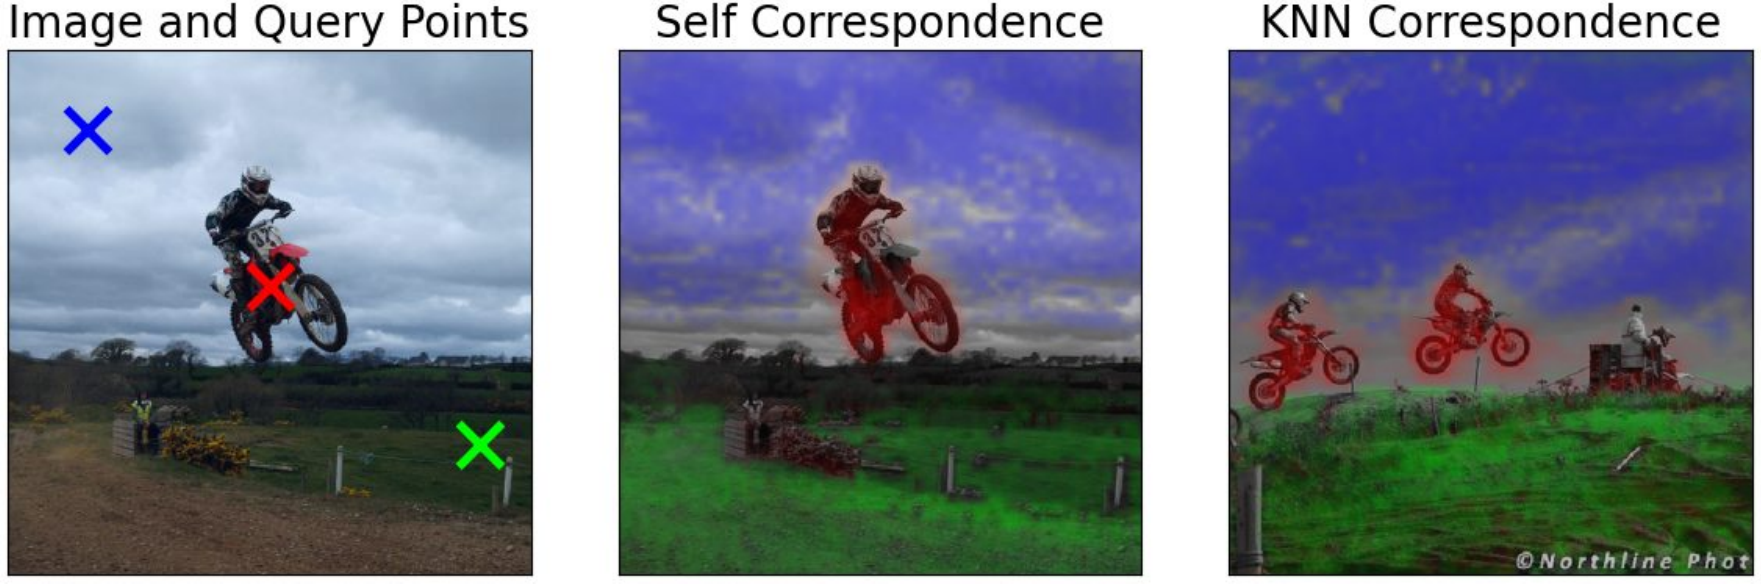
\includegraphics[width=\textwidth]{pictures/stego-feature-correspondence}\\
    \caption[Feature Correspondence of Two Images]{Feature correspondences from DINO. Correspondences between the source image (left) and the target images (middle and right) are plotted over the target images in the respective color of the source point (crosses in the left image). Feature correspondences can highlight key aspects of shared semantics within a single image (middle) and across similar images such as one of the k nearest neighbours (KNNs) (right). Figure and caption from~\autocite{Hamilton2022}.}
    \label{fig:stego-feature-correspondence}
\end{figure}

The feature correspondence signal $F_{hwij}$ can be used for high quality semantic segmentation by comparing it with the segmentation correspondence tensor $S_{hwij}$, which is calculated respectively (see~\autoref{eq:correspondence}).
The loss function aims at pushing the segmentation tensors together, when the feature tensors were found to have stronger correlation.
Additionally, zero clamping and spatial centering is applied, to hinder collapse and to balance the learning signal for small objects respectively.~\autocite{Hamilton2022}

The correspondence loss function of two images ($x$, $y$) thus is:
\begin{equation}
    L_{corr}(x,y,b) = -\sum_{hwij}\left(\underbrace{\left(F_{hwij} -\frac{1}{IJ} \sum_{i'j'}F_{hwi'j'}\right)}_{\substack{\text{spacial centered} \\ \text{correspondence loss}}}- b\right) {} \underbrace{max(S_{hwij}, 0)}_{\substack{\text{zero clamped}\\\text{segmentation} \\ \text{correspondence}}}
    \label{eq:corr-loss}
\end{equation}
Where $b$ is a negative pressure to again avoid collapse, $h,w$ are positions of image $x$ and $i,j$ positions of image $y$.
$I,J$ represent spatial dimensions.
This loss function will administer a repulsive or attractive force on the segmentation features, proportional on their feature correspondence.
The function $L_{corr}$ was shown to be a Potts model, an energy-based graph optimisation model, hence the name of \gls{stego}.~\autocite{Hamilton2022}

\gls{stego} uses three instances of the correspondence loss as final loss function to train the segmentation head: one between the image and itself, one between the image and one of its k-nearest neighbours\footnote{It was found by the authors that selecting from the seven nearest neighbours yields good results.} (both of these exerting an attractive force), and one instance between the image and five random other images, exerting a repulsive force.
To balance the negative and positive signals, weight parameters $\lambda$ are used.~\autocite{Hamilton2022}

The loss function optimised in the segmentation head thus is:
\begin{equation}
\begin{aligned}    
    L = {} & \lambda_{self}L_{corr}(x,x,b_{self}) \\
        & + \lambda_{knn}L_{corr}(x,x^{knn},b_{knn}) \\
        & + \lambda_{self}L_{rand}(x,x^{rand},b_{rand})
    \label{eq:stego-loss}
\end{aligned}
\end{equation}

In practice the authors recommend a ratio of $\lambda_{self} \approx \lambda_{knn} \approx 2 \lambda_{random}$, while the $b$s need to be tuned on a per-data-set basis, usually optimised to balance the mean knn feature similarity at $\approx 0.3$ and mean random similarity at $\approx 0.0$\footnote{This can be achieved by monitoring the provided TensorBoard (especially the variables \posinter and \neginter).}. % mean self similarity should always be at 1? depends on corpping and dataset...
However, as seen in the appendix of the paper, other weight relations were also found beneficial for different data sets.~\autocite{Hamilton2022}

\subsection{Potential and Problems}
%evaluation (calculating precision and recall)
%Since the feature correspondence is strongly correlated with the true label co-occurrence tensor $LCo$, it can be used to evaluate feature compatibility in regard to semantic segmentation using, by predicting the label co-occurrence.
%By examining how well the feature correspondence $F$ can predict the label co-occurrence $LCo$ a measure on the compatibility of the features withe the ground truth labels is found (precision and recall).
%\begin{equation}
%    LCo_{hwij} =  \begin{cases}
%                      1, & \text{if~} l_{hw} = k_{ij} \\
%                      0, & \text{if~} l_{hw} \neq k_{ij}]
%                \end{cases}
%    \label{eq:label-coocurrence}
%\end{equation}
%If two ground truth labels $l$ and $k$ are the same, label co-occurrence is 1, else label co-occurrence is 0.

% performance is very good
The authors found, that this feature distillation process did in fact significantly improve the performance in comparison to directly clustering the unmodified features the backbone provides.
In the best scenario, \gls{stego} improved the prior state-of-the-art by 9 to 14~points on the \gls{miou}~\autocite{Hamilton2022}.
Additionally, training is very fast, since the backbone is frozen with pre-trained weights provided by \gls{dino}, and only the lightweight segmentation head is trained~\autocite{Hamilton2022}.

By providing extensive configuration files, the authors allow users of \gls{stego} to adjust the network to their specific use cases.
For example, resolution and batch size can be adjusted to the image size in the train set, and different cropping methods are provided to pre-process images to account for more details in the pictures.\footnote{With the data sets used in the paper, five cropping (as explained before) was found most beneficial, but a random cropping utility is available too, which might be beneficial for different data sets.~\autocite{Ji2019}}
For training, different (pre-trained) backbones can be selected, and even completely new backbones can be integrated, once more promising candidates become available or are trained on a specific data set.~\autocite{Hamilton2022}

Additionally, training can be done with extra clusters to enable overclustering~\autocite{Hamilton2022}.
Overclustering refers to the practice of clustering with more clusters than ground truth labels.
It was theorised by~\autocite{VanGansbeke2021}, that improvement through overclustering could be attributed to the fact that pixels of the same (or visually similar) objects are found in local neighborhoods in the embedding space of models.
More practically, it can also be assumed, that allowing multiple clusters for a ground truth label, that encompasses different textures, can increase overall performance.

% (transition) but some problems when used for scientific data
However, \gls{stego} (as well as its backbone) was adapted for 2D RGB photographs~\autocite{Hamilton2022}.
This means for training 3D high-resolution grey value images, as often found in scientific imaging, some adjustments need to be made.
Additionally, it was found, that some functionalities provided in the code base did not work as intended, and needed fixing~\autocite{mhamilton7232022}.
Overall, this means, the method was not yet ready to use when downloaded from GitHub~\autocite{mhamilton7232022}, and some adaptions and corrections needed to be made before using it.
